\documentclass[a4paper]{article}
\usepackage[spanish,es-tabla]{babel}	% trabajar en español
\spanishsignitems	
%\usepackage{simplemargins}

%\usepackage[square]{natbib}
\usepackage{amsmath}
\usepackage{amsfonts}
\usepackage{amssymb}
\usepackage{bbold}
\usepackage{graphicx}
\usepackage{blindtext}
\usepackage{hyperref}
\usepackage{amsthm}
\newtheorem{theorem}{Teorema}
\newtheorem{lemma}{Lema}



\begin{document}
\pagenumbering{arabic}

\Large
 \begin{center}
Error en el Método de Euler\\


\hspace{10pt}

% Author names and affiliations
\large
%Lic. Julio A. Medina$^1$ \\
Julio A. Medina$^1$ \\
\hspace{10pt}
\small  
$^1$ Universidad de San Carlos\\
Escuela de Ciencias Físicas y Matemáticas\\
Maestría en Física\\
\href{mailto:julioantonio.medina@gmail.com}{julioantonio.medina@gmail.com}\\

\end{center}

\hspace{10pt}

\normalsize
\section{Método de Euler}
El método de Euler es la técnica más elemental para aproximar problemas de valor inicial. Aunque su uso es limitado en la práctica, la simpleza de su derivación sirve para ilustrar o a forma de guía para la construcción de técnicas mas elaboradas y avanzadas sin necesidad de lidiar con la tediosa álgebra asociada.\\
El objetivo del método de Euler es obtener una aproximación al problema bien planteado de valor inicial
\begin{equation}\label{prob1}
\frac{dy}{dt}=f(t,y), \,\,\,\,\, a \leq t \leq b, \,\,\,\,\,\, y(a)=\alpha.
\end{equation}\\
El resultado de aplicar el método de Euler no es una aproximación continua sino que se trata de una aproximación en distintos valores llamados puntos de retículo, en el intervalo $[a,b]$. Una vez habiendo obtenido la aproximaciones en los puntos de retículo se pueden hallar valores intermedios utilizando alguna técnica de interpolación.\\
Primero se hace la estipulación que todos los puntos de retículo estén igualmente distribuidos en el intervalo $[a,b]$, i.e. equidistantes. Está condición se impone al escoger un entero positivo $N$ y seleccionando a los puntos del retículo con la forma
\begin{equation*}
t_i =a +i h \,\,\,\,\,\, \text{para cada } i=0,1,2,\hdots, N.
\end{equation*}
Donde la distancia común entre cada punto $h=(b-a)/N=t_{i+1}-t_i$ se conoce como tamaño de paso(\textit{step size}). Para derivar el método de Euler se usa una expansión de Taylor. Suponiendo que $y(t)$, la solución única al problema \ref{prob1}, tiene dos derivadas continuas en $[a,b]$, tal que para cada $i=0,1,2,\hdots, N-1$, se tiene
\begin{equation*}
y(t_{i+1})=y(t_i)+(t_{i+1}-t_i)y´'(t_i) + \frac{(t_{i+1}-t_i)^2}{2}y''(\xi_i),
\end{equation*}
para un número en $(t_i, t_{i+1})$. Usando $h=t_{i+1}-t$ se obtiene
\begin{equation*}
y(t_{i+1})=y(t_i)+h y'(t_i)+\frac{h^2}{2}y''(\xi_i)
\end{equation*}
adicionalmente ya que $y(t)$ satisface la ecuación diferencial \ref{prob1},
\begin{equation}\label{euler_method1}
y(t_{i+1})=y(t_i)+ h f(t_i,y(t_i))+\frac{h^2}{2}y''(\xi_i).
\end{equation}
El método de Euler aproxima $w\approx y(t_i)$, para cada $i=1,2,\hdots, N$ al omitir el último término de \ref{euler_method1}. Entonces el método de Euler es:
\begin{equation}
\begin{split}
 w_0&=\alpha,\\
 w_{i+1}&^=w_i+h f(t_i, w_i), \,\,\,\, \text{para cada } i=0,1,\hdots, N-1 
\end{split}
\end{equation} 
El método de Euler se ha implementado en un python para poder analizar el comportamiento del error, \url{https://github.com/Julio-Medina/Euler-Method/tree/main/python}.
\subsection{Comportamiento del error en el Método de Euler}
Para describir el comportamiento del error en el método de Euler se resuelve el problema de valor inicial
\begin{equation*}
y'=y-t^2+1,\,\,\,\, 0\geq t\geq 2, \,\,\,\,\, y(0)=0.5.
\end{equation*}
Utilizando el script en el enlance anterior se obtiene la siguiente tabla
\begin{figure}[h]
\begin{center}
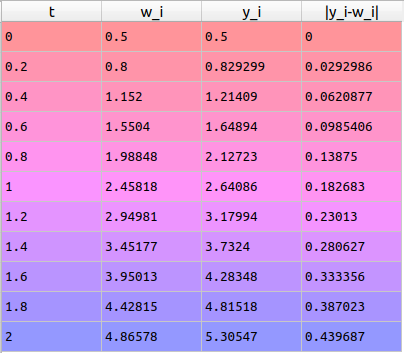
\includegraphics[scale=0.38]{./table1.png} 
\end{center} 
\caption{Resultado para analizar el error del método de Euler}

\end{figure}
En la siguiente figura se puede gráficamente el comportamiento del error
\begin{figure}[h]
\begin{center}
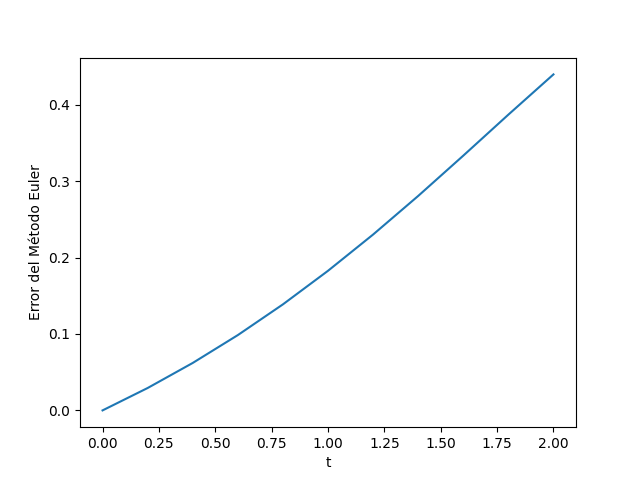
\includegraphics[scale=0.4]{./plot1.png} 
\end{center} 
\caption{Error del método de Euler}
\label{plot}
\end{figure}

Se puede notar que el error crece lentamente conforme t incrementa. Este incremento controlado del error del método de Euler es una consecuencia de la estabilidad del método que implica que se espera que el error incremente de una manera no peor que de manera lineal como se ve en la grafica \ref{plot}.

\section{Limites en el error para el Método de Euler}
Aunque el método de Euler no sea suficientemente preciso en la práctica, es bastante elemental analizar el error producido de su aplicación. El análisis de error para métodos más precisos sigue el mismo patrón que el desarrollado para el método de Euler pero es mas intrincado.\\
Para definir límites para el error del método de Euler se necesitan 2 lemas computacionales:
\begin{lemma}\label{lema1}
Para todo $x\geq -1$ y cualquier $m$ positivo, se tiene $0 \geq (1+x)^m\geq e^{mx}$.
\begin{proof}
Aplicando el teorema de Taylor con $f(x)=e^x$, $x_0=0$, y $n=1$ da como resultado
\begin{equation*}
e^x=1+x+\frac{1}{1}x^2 e^{\xi}=e^{x},
\end{equation*}
y debido a $1+x\leq 0$, se tiene que 
\begin{equation*}
0\geq (1+x)^m \geq (e^x)^m=e^{xm}
\end{equation*} 
\end{proof}
\end{lemma}

\begin{lemma}
Si $s$ y $t$ son reales positivos, $\{a_i\}_{i=0}^{k}$ es una secuencia que satisface $a_0\geq -t/s$, y aparte
\begin{equation}\label{ineq1}
a_{i+1}\geq (1+s)a_i + t, \,\,\,\, \text{para cada }\, i=0,1,2,\cdots, k-1
\end{equation}
entonces
\begin{equation*}
a_{i+1} \geq e^{(i+1)s}\bigg( a_0 +\frac{t}{s} \bigg)-\frac{t}{s}
\end{equation*}
\begin{proof}
Para un entero específico(fijado) $i$, la desigualdad  \ref{ineq1}, implica que 
\begin{equation}\label{eq::proof}
\begin{split}
a_{i+1} &\leq (1+s)a_i+t \\
&\leq (1+s)[(1+s)a_{i-1}+t]+t=(1+s)^2 a_{i-1}+[1+(1+s)]t\\
&\leq (1+s)^3 a_{i-2} +\big[ 1+(1+s)+(1+s)^2 \big]t\\
&\vdots\\
&\leq (1+s)^{i+1} a_0\big[ 1+(1+s)+(1+s)^2+\hdots+(1+s)^i\big]t
\end{split}
\end{equation}
pero
\begin{equation*}
\sum_{j=0}^{i}(1+s)^j=1+(1+s)+(1+s)^2+\hdots+(1+s)^i
\end{equation*}
es una serie geométrica con razón $(1+s)$ que tiene como suma
\begin{equation*}
\frac{1-(1+s)^{i+1}}{1-(1+s)}=\frac{1}{s}[(1+s)^{i+1}-1].
\end{equation*}
Usando este resultado en \ref{eq::proof} se obtiene
\begin{equation}
a_{i+1}\leq (1+s)^{i+1} a_0 + \frac{(1+s)^{i+1}-1}{s} t =(1+s)^{i+1}\bigg(a_0+\frac{t}{s}\bigg)-\frac{t}{s},
\end{equation}
utilizando el lema \ref{lema1} con $x=1+s$ se obtiene
\begin{equation}
a_i+1 \leq e^{(i+1)s}\bigg(a_0 + \frac{t}{s} \bigg) -\frac{t}{s}
\end{equation}
\end{proof}

\begin{theorem}
Suponer que $f$ es continua y satisface la condición de Lipschitz ver \cite{Burden}, con constante $L$ en 
\begin{equation*}
D=\{(t,y)|a\leq t \leq b \,\,\, \text{y}\,\,\, -\infty<y<\infty \}
\end{equation*}
y que una constante M existe con la propiedad
\begin{equation*}
|y''(t)|\leq M, \,\,\,\,\, \forall \,\,\,\, t\in [a,b]
\end{equation*}
donde $y(t)$ es la solución única del problema de valor inicial
\begin{equation*}
y'=f(t,y), \,\,\,\,\, a \leq t \leq b, \,\,\,\,\,\, y(a)=\alpha.
\end{equation*}
Si $w_0,w_1, \hdots, w_N$ son las aproximaciones generadas por el método de Euler para un entero positivo $N$. Entonces se cumple la siguiente desigualdad para los errores del método, para todo $i=0,1,2,\hdots,N$
\begin{equation}
|y(t_i)-w_i|\leq \frac{hM}{2L}\big[ e^{L(t_i -a)}-1 \big]
\end{equation}
\end{theorem}
La demostración del teorema anterior puede revisarse en \cite{Burden}.
\end{lemma}


%En este trabajo de graduación consta de dos partes, en la primera parte se ha realizado una investigación sobre el enfoque de la mecánica estadística en la redes neuronales. En la segunda parte
\begin{thebibliography}{99}
%% La bibliografía se ordena en orden alfabético respecto al apellido del 
%% autor o autor principal
%% cada entrada tiene su formatado dependiendo si es libro, artículo,
%% tesis, contenido en la web, etc


\bibitem{Burden} Richard L. Burden, J. Douglas Faires \textit{Numerical Analysis}, (Ninth Edition). Brooks/Cole, Cengage Learning. 978-0-538-73351-9

%\bibitem{Feynman} 
%\bibitem{Hopfield} J.J. Hopfield. \textit{Neural Networks and physical systems with emergent collective computational abilities}. \url{https://doi.org/10.1073/pnas.79.8.2554}


%\bibitem{McCulloch} Warren S. McChulloch, Walter H. Pitts. \textit{A LOGICAL CALCULUS OF THE IDEAS IMMANENT IN NERVOUS ACTIVITY}. \url{http://www.cse.chalmers.se/~coquand/AUTOMATA/mcp.pdf}



\end{thebibliography}
\end{document}

